\documentclass[]{tufte-handout}

% ams
\usepackage{amssymb,amsmath}

\usepackage{ifxetex,ifluatex}
\usepackage{fixltx2e} % provides \textsubscript
\ifnum 0\ifxetex 1\fi\ifluatex 1\fi=0 % if pdftex
  \usepackage[T1]{fontenc}
  \usepackage[utf8]{inputenc}
\else % if luatex or xelatex
  \makeatletter
  \@ifpackageloaded{fontspec}{}{\usepackage{fontspec}}
  \makeatother
  \defaultfontfeatures{Ligatures=TeX,Scale=MatchLowercase}
  \makeatletter
  \@ifpackageloaded{soul}{
     \renewcommand\allcapsspacing[1]{{\addfontfeature{LetterSpace=15}#1}}
     \renewcommand\smallcapsspacing[1]{{\addfontfeature{LetterSpace=10}#1}}
   }{}
  \makeatother

\fi

% graphix
\usepackage{graphicx}
\setkeys{Gin}{width=\linewidth,totalheight=\textheight,keepaspectratio}

% booktabs
\usepackage{booktabs}

% url
\usepackage{url}

% hyperref
\usepackage{hyperref}

% units.
\usepackage{units}


\setcounter{secnumdepth}{-1}

% citations
\usepackage{natbib}
\bibliographystyle{plainnat}


% pandoc syntax highlighting
\usepackage{color}
\usepackage{fancyvrb}
\newcommand{\VerbBar}{|}
\newcommand{\VERB}{\Verb[commandchars=\\\{\}]}
\DefineVerbatimEnvironment{Highlighting}{Verbatim}{commandchars=\\\{\}}
% Add ',fontsize=\small' for more characters per line
\newenvironment{Shaded}{}{}
\newcommand{\AlertTok}[1]{\textcolor[rgb]{1.00,0.00,0.00}{\textbf{#1}}}
\newcommand{\AnnotationTok}[1]{\textcolor[rgb]{0.38,0.63,0.69}{\textbf{\textit{#1}}}}
\newcommand{\AttributeTok}[1]{\textcolor[rgb]{0.49,0.56,0.16}{#1}}
\newcommand{\BaseNTok}[1]{\textcolor[rgb]{0.25,0.63,0.44}{#1}}
\newcommand{\BuiltInTok}[1]{#1}
\newcommand{\CharTok}[1]{\textcolor[rgb]{0.25,0.44,0.63}{#1}}
\newcommand{\CommentTok}[1]{\textcolor[rgb]{0.38,0.63,0.69}{\textit{#1}}}
\newcommand{\CommentVarTok}[1]{\textcolor[rgb]{0.38,0.63,0.69}{\textbf{\textit{#1}}}}
\newcommand{\ConstantTok}[1]{\textcolor[rgb]{0.53,0.00,0.00}{#1}}
\newcommand{\ControlFlowTok}[1]{\textcolor[rgb]{0.00,0.44,0.13}{\textbf{#1}}}
\newcommand{\DataTypeTok}[1]{\textcolor[rgb]{0.56,0.13,0.00}{#1}}
\newcommand{\DecValTok}[1]{\textcolor[rgb]{0.25,0.63,0.44}{#1}}
\newcommand{\DocumentationTok}[1]{\textcolor[rgb]{0.73,0.13,0.13}{\textit{#1}}}
\newcommand{\ErrorTok}[1]{\textcolor[rgb]{1.00,0.00,0.00}{\textbf{#1}}}
\newcommand{\ExtensionTok}[1]{#1}
\newcommand{\FloatTok}[1]{\textcolor[rgb]{0.25,0.63,0.44}{#1}}
\newcommand{\FunctionTok}[1]{\textcolor[rgb]{0.02,0.16,0.49}{#1}}
\newcommand{\ImportTok}[1]{#1}
\newcommand{\InformationTok}[1]{\textcolor[rgb]{0.38,0.63,0.69}{\textbf{\textit{#1}}}}
\newcommand{\KeywordTok}[1]{\textcolor[rgb]{0.00,0.44,0.13}{\textbf{#1}}}
\newcommand{\NormalTok}[1]{#1}
\newcommand{\OperatorTok}[1]{\textcolor[rgb]{0.40,0.40,0.40}{#1}}
\newcommand{\OtherTok}[1]{\textcolor[rgb]{0.00,0.44,0.13}{#1}}
\newcommand{\PreprocessorTok}[1]{\textcolor[rgb]{0.74,0.48,0.00}{#1}}
\newcommand{\RegionMarkerTok}[1]{#1}
\newcommand{\SpecialCharTok}[1]{\textcolor[rgb]{0.25,0.44,0.63}{#1}}
\newcommand{\SpecialStringTok}[1]{\textcolor[rgb]{0.73,0.40,0.53}{#1}}
\newcommand{\StringTok}[1]{\textcolor[rgb]{0.25,0.44,0.63}{#1}}
\newcommand{\VariableTok}[1]{\textcolor[rgb]{0.10,0.09,0.49}{#1}}
\newcommand{\VerbatimStringTok}[1]{\textcolor[rgb]{0.25,0.44,0.63}{#1}}
\newcommand{\WarningTok}[1]{\textcolor[rgb]{0.38,0.63,0.69}{\textbf{\textit{#1}}}}

% longtable

% multiplecol
\usepackage{multicol}

% strikeout
\usepackage[normalem]{ulem}

% morefloats
\usepackage{morefloats}


% tightlist macro required by pandoc >= 1.14
\providecommand{\tightlist}{%
  \setlength{\itemsep}{0pt}\setlength{\parskip}{0pt}}

% title / author / date
\title[標本平均を用いた変動は必ず小さくなるのか?]{標本平均を用いた変動は必ず小さくなるか?}
\author{Sampo Suzuki, CC 4.0 BY-NC-SA}
\date{2021-06-29}

% --- 参考資料 ----------------------------------------------------------------
% http://ctan.math.illinois.edu/language/japanese/zxjafont/zxjafont.pdf
% https://github.com/Gedevan-Aleksizde/Japan.R2019/blob/master/latex/preamble.tex
% https://teastat.blogspot.com/2019/01/bookdown.html

% --- Packages ----------------------------------------------------------------
% 日本語とtufte, kableExtraを使うために必要なTeXパッケージ指定
% \usepackage[pdfbox,tombo]{gentombow}    % トンボを設定する場合は有効にする
\usepackage{ifthen}                     % 条件分岐用 \ifthenelse{条件}{T}{F}
\usepackage{booktabs}                   % ここからkableExtra用パッケージ
\usepackage{longtable}                  % 
\usepackage{array}                      % 
\usepackage{multirow}                   % 
\usepackage{wrapfig}                    % 
\usepackage{float}                      % 
\usepackage{colortbl}                   % 
\usepackage{pdflscape}                  % 
\usepackage{tabu}                       % 
\usepackage{threeparttable}             % 
\usepackage{threeparttablex}            % 
\usepackage[normalem]{ulem}             % 
\usepackage{inputenc}                   % 
\usepackage{makecell}                   % 
\usepackage{xcolor}                     % ここまでkableExtra用
\usepackage{amsmath}                    % 
\usepackage{fontawesome5}               % fontawesomeを使うために必要
\usepackage{subfig}                     % 複数の図を並べる際に必要(古い?)
% \usepackage{subcaption}                 % 同上(新しい?)
\usepackage{zxjatype}                   % 日本語処理に必要
% \usepackage{xeCJK}                      % zxjatypeを読み込むと一緒に読み込まれる
\usepackage[noto]{zxjafont}             % Linux環境用
% \usepackage[haranoaji]{zxjafont}        % Windows環境用
% \usepackage[hiragino-pro]{zxjafont}     % macOS環境用(おそらく、駄目ならNotoで)
\usepackage{pxrubrica}                  % ルビ用
\usepackage{hyperref}                   % ハイパーリンク用必要?
% 以下のパッケージについては下記サイトを参照方
% http://www.yamamo10.jp/yamamoto/comp/latex/make_doc/box/box.php
% \usepackage{ascmac}                     % 別行で文書を囲む場合
% \usepackage{fancybox}                   % 行中で文書を囲む場合 fancybx ではない
% \usepackage{fancyhdr}                   % ヘッダー用

% https://ja.wikibooks.org/wiki/TeX/LaTeX%E5%85%A5%E9%96%80
% https://teastat.blogspot.com/2019/01/bookdown.html
\usepackage{booktabs}
\usepackage{longtable}
\usepackage{array}
\usepackage{multirow}
\usepackage{wrapfig}
\usepackage{float}
\usepackage{colortbl}
\usepackage{pdflscape}
\usepackage{tabu}
\usepackage{threeparttable}
\usepackage{threeparttablex}
\usepackage[normalem]{ulem}
\usepackage{makecell}
\usepackage{xcolor}

\begin{document}

\maketitle




\hypertarget{ux6a19ux672cux5e73ux5747ux3092ux7528ux3044ux305fux5909ux52d5ux306fux5fc5ux305aux5c0fux3055ux304fux306aux308bux306eux304b}{%
\section{\texorpdfstring{\textbf{標本平均を用いた変動は必ず小さくなるのか?}}{標本平均を用いた変動は必ず小さくなるのか?}}\label{ux6a19ux672cux5e73ux5747ux3092ux7528ux3044ux305fux5909ux52d5ux306fux5fc5ux305aux5c0fux3055ux304fux306aux308bux306eux304b}}

 『ソフトウェアメトリクス統計分析入門』\citep{SoftwareMetrics:jbook}の3.3
ワンポイント講義「不偏分散を算出する際に自由度を用いる理由」には、標本平均(\(\bar{x}\))を使って算出した変動(\(\sum_{i = 1}^{n}(x_i - \bar{x})^2\)、偏差平方和)は母平均(\(\mu\))を使って算出した変動(\(\sum_{i = 1}^{n}(x_i - \mu)^2\))よりも必ず小さな値になるとあります。実際に小さくなるのかを確認します。

\hypertarget{ux6bcdux96c6ux56e3ux30c7ux30fcux30bfux306eux4f5cux6210}{%
\subsection{\texorpdfstring{\textbf{母集団データの作成}}{母集団データの作成}}\label{ux6bcdux96c6ux56e3ux30c7ux30fcux30bfux306eux4f5cux6210}}

 最初に正規分布を持つ母集団のデータ(\(x\))を作成します。ここでは母平均と母標準偏差は不明であると仮定します。

\begin{figure}

{\centering 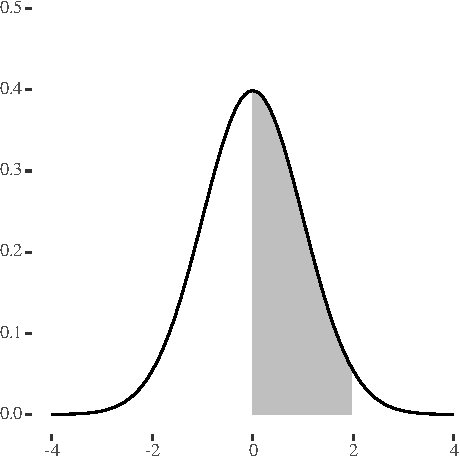
\includegraphics[width=0.8\linewidth]{DegreeOfFreedum_files/figure-latex/unnamed-chunk-1-1} 

}

\caption[母集団の分布]{母集団の分布}\label{fig:unnamed-chunk-1}
\end{figure}

\newpage

\hypertarget{ux7c21ux5358ux306aux30b7ux30dfux30e5ux30ecux30fcux30b7ux30e7ux30f3}{%
\subsection{\texorpdfstring{\textbf{簡単なシミュレーション}}{簡単なシミュレーション}}\label{ux7c21ux5358ux306aux30b7ux30dfux30e5ux30ecux30fcux30b7ux30e7ux30f3}}

 上記の母集団(\(x\))から以下の手順で二種類の変動(偏差平方和)を求めます。

\begin{enumerate}
\def\labelenumi{\arabic{enumi}.}
\tightlist
\item
  3つのデータをランダムサンプリングで取り出す(標本
  \(x_n, n = 1, 2, 3\))
\item
  取り出したデータの平均値(標本平均 \(\bar{x}\))を求める
\item
  標本平均(\(\bar{x}\))を用いて標本の変動(偏差平方和
  \(\sum_{i = 1}^{n}(x_i - \bar{x})^2\))を求める
\item
  母平均(\(\mu\))を用いて標本の変動(偏差平方和
  \(\sum_{i = 1}^{n}(x_i - \mu)^2\))を求める
\item
  求めた二つの変動(偏差平方和)を比較する
\end{enumerate}

この計算を任意の回数繰り返して標本平均(\(\bar{x}\))を用いた標本の変動(偏差平方和
\(\sum_{i = 1}^{n}(x_i - \bar{x})^2\))の方が小さいことを確認します。

\begin{Shaded}
\begin{Highlighting}[numbers=left,,]
\NormalTok{df }\OtherTok{\textless{}{-}} \FunctionTok{data.frame}\NormalTok{()}
\ControlFlowTok{for}\NormalTok{ (i }\ControlFlowTok{in} \FunctionTok{c}\NormalTok{(}\DecValTok{1}\SpecialCharTok{:}\DecValTok{30}\NormalTok{)) \{}
\NormalTok{  xs }\OtherTok{\textless{}{-}} \FunctionTok{sample}\NormalTok{(x, }\AttributeTok{size =} \DecValTok{3}\NormalTok{, }\AttributeTok{replace =} \ConstantTok{FALSE}\NormalTok{)  }\CommentTok{\# 母集団から3つのデータを取り出す}
\NormalTok{  xb }\OtherTok{\textless{}{-}} \FunctionTok{mean}\NormalTok{(xs)                  }\CommentTok{\# 標本平均を求める}
\NormalTok{  dssxb }\OtherTok{\textless{}{-}} \FunctionTok{sum}\NormalTok{((xs }\SpecialCharTok{{-}}\NormalTok{ xb)}\SpecialCharTok{\^{}}\DecValTok{2}\NormalTok{)       }\CommentTok{\# 標本平均を用いた変動(偏差平方和)}
\NormalTok{  dssmu }\OtherTok{\textless{}{-}} \FunctionTok{sum}\NormalTok{((xs }\SpecialCharTok{{-}}\NormalTok{ mu)}\SpecialCharTok{\^{}}\DecValTok{2}\NormalTok{)       }\CommentTok{\# 母平均を用いた変動(偏差平方和)}
  \CommentTok{\# 計算結果をデータフレームにまとめる}
\NormalTok{  dftmp }\OtherTok{\textless{}{-}} \FunctionTok{data.frame}\NormalTok{(}\AttributeTok{no =}\NormalTok{ i,     }\CommentTok{\# 通し番号}
                      \AttributeTok{x1 =}\NormalTok{ xs[}\DecValTok{1}\NormalTok{], }\CommentTok{\# 標本データ(n = 1)}
                      \AttributeTok{x2 =}\NormalTok{ xs[}\DecValTok{2}\NormalTok{], }\CommentTok{\# 標本データ(n = 2)}
                      \AttributeTok{x3 =}\NormalTok{ xs[}\DecValTok{3}\NormalTok{], }\CommentTok{\# 標本データ(n = 3)}
\NormalTok{                      xb,         }\CommentTok{\# 標本平均}
\NormalTok{                      mu,         }\CommentTok{\# 母平均}
\NormalTok{                      dssxb,      }\CommentTok{\# 標本平均を用いた変動(偏差平方和)}
\NormalTok{                      dssmu,      }\CommentTok{\# 母平均を用いた変動(偏差平方和)}
                      \AttributeTok{diff =}\NormalTok{ dssxb }\SpecialCharTok{{-}}\NormalTok{ dssmu  }\CommentTok{\# 負値なら標本平均による変動が小さい}
\NormalTok{                      )}
\NormalTok{  df }\OtherTok{\textless{}{-}}\NormalTok{ dplyr}\SpecialCharTok{::}\FunctionTok{bind\_rows}\NormalTok{(df, dftmp)}
\NormalTok{\}}

\NormalTok{df }\SpecialCharTok{\%\textgreater{}\%} 
\NormalTok{  dplyr}\SpecialCharTok{::}\FunctionTok{rename}\NormalTok{(}\StringTok{\textasciigrave{}}\AttributeTok{標本平均}\StringTok{\textasciigrave{}}\OtherTok{=}\NormalTok{ xb, }\StringTok{\textasciigrave{}}\AttributeTok{母平均}\StringTok{\textasciigrave{}} \OtherTok{=}\NormalTok{ mu,}
                \StringTok{\textasciigrave{}}\AttributeTok{標本平均での変動}\StringTok{\textasciigrave{}} \OtherTok{=}\NormalTok{ dssxb, }\StringTok{\textasciigrave{}}\AttributeTok{母平均での変動}\StringTok{\textasciigrave{}} \OtherTok{=}\NormalTok{ dssmu,}
                \StringTok{\textasciigrave{}}\AttributeTok{変動差(標本{-}母)}\StringTok{\textasciigrave{}} \OtherTok{=}\NormalTok{ diff) }\SpecialCharTok{\%\textgreater{}\%} 
  \FunctionTok{df\_print}\NormalTok{(}\AttributeTok{all =} \ConstantTok{TRUE}\NormalTok{, }\AttributeTok{scale\_down =} \ConstantTok{TRUE}\NormalTok{, }\AttributeTok{caption =} \StringTok{"シミュレーション結果"}\NormalTok{)}
\end{Highlighting}
\end{Shaded}

\begin{table}

\caption{\label{tab:unnamed-chunk-2}シミュレーション結果}
\centering
\resizebox{\linewidth}{!}{
\begin{tabular}[t]{rrrrrrrrr}
\toprule
no & x1 & x2 & x3 & 標本平均 & 母平均 & 標本平均での変動 & 母平均での変動 & 変動差(標本-母)\\
\midrule
\cellcolor{gray!6}{1} & \cellcolor{gray!6}{2.9498361} & \cellcolor{gray!6}{4.8030369} & \cellcolor{gray!6}{5.376113} & \cellcolor{gray!6}{4.3763286} & \cellcolor{gray!6}{3.984684} & \cellcolor{gray!6}{3.2165290} & \cellcolor{gray!6}{3.676686} & \cellcolor{gray!6}{-0.4601569}\\
2 & 2.9422607 & 3.7882078 & 2.046987 & 2.9258186 & 3.984684 & 1.5163296 & 4.879916 & -3.3635863\\
\cellcolor{gray!6}{3} & \cellcolor{gray!6}{-1.3890396} & \cellcolor{gray!6}{6.1825887} & \cellcolor{gray!6}{2.102006} & \cellcolor{gray!6}{2.2985182} & \cellcolor{gray!6}{3.984684} & \cellcolor{gray!6}{28.7227028} & \cellcolor{gray!6}{37.252166} & \cellcolor{gray!6}{-8.5294631}\\
4 & 5.4850067 & 2.8509317 & 2.114541 & 3.4834930 & 3.984684 & 6.2802215 & 7.033798 & -0.7535766\\
\cellcolor{gray!6}{5} & \cellcolor{gray!6}{4.1080593} & \cellcolor{gray!6}{4.9947869} & \cellcolor{gray!6}{1.860016} & \cellcolor{gray!6}{3.6542875} & \cellcolor{gray!6}{3.984684} & \cellcolor{gray!6}{5.2222560} & \cellcolor{gray!6}{5.549741} & \cellcolor{gray!6}{-0.3274851}\\
\addlinespace
6 & 9.0280057 & -3.1743646 & 5.726024 & 3.8598883 & 3.984684 & 79.6726125 & 79.719334 & -0.0467218\\
\cellcolor{gray!6}{7} & \cellcolor{gray!6}{6.5385761} & \cellcolor{gray!6}{8.0532167} & \cellcolor{gray!6}{1.003216} & \cellcolor{gray!6}{5.1983363} & \cellcolor{gray!6}{3.984684} & \cellcolor{gray!6}{27.5456179} & \cellcolor{gray!6}{31.964475} & \cellcolor{gray!6}{-4.4188573}\\
8 & 5.9855130 & 4.0936488 & 2.889727 & 4.3229631 & 3.984684 & 4.8708215 & 5.214120 & -0.3432987\\
\cellcolor{gray!6}{9} & \cellcolor{gray!6}{3.9842593} & \cellcolor{gray!6}{-0.9345524} & \cellcolor{gray!6}{11.697489} & \cellcolor{gray!6}{4.9157320} & \cellcolor{gray!6}{3.984684} & \cellcolor{gray!6}{81.0857001} & \cellcolor{gray!6}{83.686252} & \cellcolor{gray!6}{-2.6005523}\\
10 & 2.6566400 & 2.6948555 & 3.363902 & 2.9051324 & 3.984684 & 0.3164341 & 3.812728 & -3.4962937\\
\addlinespace
\cellcolor{gray!6}{11} & \cellcolor{gray!6}{4.3832517} & \cellcolor{gray!6}{4.1297346} & \cellcolor{gray!6}{4.668041} & \cellcolor{gray!6}{4.3936757} & \cellcolor{gray!6}{3.984684} & \cellcolor{gray!6}{0.1450498} & \cellcolor{gray!6}{0.646873} & \cellcolor{gray!6}{-0.5018232}\\
12 & 1.1831673 & 6.0825864 & -5.135020 & 0.7102445 & 3.984684 & 63.2528323 & 95.418691 & -32.1658587\\
\cellcolor{gray!6}{13} & \cellcolor{gray!6}{4.0711975} & \cellcolor{gray!6}{1.1562107} & \cellcolor{gray!6}{3.308821} & \cellcolor{gray!6}{2.8454097} & \cellcolor{gray!6}{3.984684} & \cellcolor{gray!6}{4.5706989} & \cellcolor{gray!6}{8.464535} & \cellcolor{gray!6}{-3.8938363}\\
14 & 4.2007156 & 4.8714447 & 1.408004 & 3.4933882 & 3.984684 & 6.7481781 & 7.472292 & -0.7241142\\
\cellcolor{gray!6}{15} & \cellcolor{gray!6}{4.5775337} & \cellcolor{gray!6}{4.0539793} & \cellcolor{gray!6}{8.293052} & \cellcolor{gray!6}{5.6415218} & \cellcolor{gray!6}{3.984684} & \cellcolor{gray!6}{10.6829771} & \cellcolor{gray!6}{18.918314} & \cellcolor{gray!6}{-8.2353368}\\
\addlinespace
16 & 4.2242886 & 7.6331796 & 0.670143 & 4.1758704 & 3.984684 & 24.2454558 & 24.355113 & -0.1096570\\
\cellcolor{gray!6}{17} & \cellcolor{gray!6}{6.0319595} & \cellcolor{gray!6}{1.6244979} & \cellcolor{gray!6}{0.282768} & \cellcolor{gray!6}{2.6464085} & \cellcolor{gray!6}{3.984684} & \cellcolor{gray!6}{18.0930536} & \cellcolor{gray!6}{23.465996} & \cellcolor{gray!6}{-5.3729427}\\
18 & 3.5105381 & 1.1650633 & 1.011195 & 1.8955989 & 3.984684 & 3.9238804 & 17.016708 & -13.0928272\\
\cellcolor{gray!6}{19} & \cellcolor{gray!6}{5.7761526} & \cellcolor{gray!6}{7.5624690} & \cellcolor{gray!6}{1.102853} & \cellcolor{gray!6}{4.8138250} & \cellcolor{gray!6}{3.984684} & \cellcolor{gray!6}{22.2524298} & \cellcolor{gray!6}{24.314855} & \cellcolor{gray!6}{-2.0624253}\\
20 & 4.8925723 & 3.2339782 & 5.755922 & 4.6274908 & 3.984684 & 3.2855024 & 4.525105 & -1.2396025\\
\addlinespace
\cellcolor{gray!6}{21} & \cellcolor{gray!6}{4.7781403} & \cellcolor{gray!6}{3.3230197} & \cellcolor{gray!6}{9.156763} & \cellcolor{gray!6}{5.7526409} & \cellcolor{gray!6}{3.984684} & \cellcolor{gray!6}{18.4407557} & \cellcolor{gray!6}{27.817773} & \cellcolor{gray!6}{-9.3770171}\\
22 & 5.1021692 & 5.6443430 & 5.256119 & 5.3342104 & 3.984684 & 0.1561236 & 5.619790 & -5.4636663\\
\cellcolor{gray!6}{23} & \cellcolor{gray!6}{5.3166644} & \cellcolor{gray!6}{2.6901232} & \cellcolor{gray!6}{3.610101} & \cellcolor{gray!6}{3.8722960} & \cellcolor{gray!6}{3.984684} & \cellcolor{gray!6}{3.5524790} & \cellcolor{gray!6}{3.590372} & \cellcolor{gray!6}{-0.0378930}\\
24 & -0.0826761 & 1.2425152 & 4.480185 & 1.8800081 & 3.984684 & 11.0194465 & 24.308427 & -13.2889801\\
\cellcolor{gray!6}{25} & \cellcolor{gray!6}{4.9519314} & \cellcolor{gray!6}{7.0017511} & \cellcolor{gray!6}{4.258477} & \cellcolor{gray!6}{5.4040532} & \cellcolor{gray!6}{3.984684} & \cellcolor{gray!6}{4.0693974} & \cellcolor{gray!6}{10.113226} & \cellcolor{gray!6}{-6.0438284}\\
\addlinespace
26 & 2.4656320 & 4.7573844 & 8.669014 & 5.2973434 & 3.984684 & 19.6783063 & 24.847532 & -5.1692257\\
\cellcolor{gray!6}{27} & \cellcolor{gray!6}{6.1788690} & \cellcolor{gray!6}{2.7941764} & \cellcolor{gray!6}{5.130989} & \cellcolor{gray!6}{4.7013448} & \cellcolor{gray!6}{3.984684} & \cellcolor{gray!6}{6.0049633} & \cellcolor{gray!6}{7.545772} & \cellcolor{gray!6}{-1.5408090}\\
28 & -0.0638104 & 4.9923238 & 5.554449 & 3.4943208 & 3.984684 & 19.1484393 & 19.869807 & -0.7213676\\
\cellcolor{gray!6}{29} & \cellcolor{gray!6}{3.5509714} & \cellcolor{gray!6}{0.8846013} & \cellcolor{gray!6}{4.057784} & \cellcolor{gray!6}{2.8311190} & \cellcolor{gray!6}{3.984684} & \cellcolor{gray!6}{5.8118266} & \cellcolor{gray!6}{9.803962} & \cellcolor{gray!6}{-3.9921351}\\
30 & 3.3666071 & -2.3742030 & 4.738442 & 1.9102821 & 3.984684 & 28.4761854 & 41.385613 & -12.9094271\\
\bottomrule
\end{tabular}}
\end{table}

\begin{figure}

{\centering 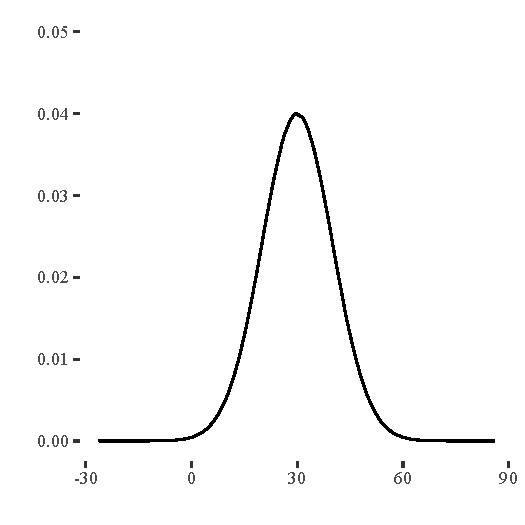
\includegraphics[width=0.8\linewidth]{DegreeOfFreedum_files/figure-latex/unnamed-chunk-3-1} 

}

\caption[標本平均を用いた変動と母平均を用いた変動の差]{標本平均を用いた変動と母平均を用いた変動の差}\label{fig:unnamed-chunk-3}
\end{figure}

\newpage

\hypertarget{ux6a19ux672cux6a19ux6e96ux504fux5deeux306eux88dcux6b63ux5024ux3092ux78baux8a8dux3059ux308b}{%
\section{\texorpdfstring{\textbf{標本標準偏差の補正値を確認する}}{標本標準偏差の補正値を確認する}}\label{ux6a19ux672cux6a19ux6e96ux504fux5deeux306eux88dcux6b63ux5024ux3092ux78baux8a8dux3059ux308b}}

 標本平均(\(\bar{x}\))を用いた変動(偏差平方和)は母平均(\(\mu\))を用いた変動(偏差平方和)よりも小さくなることがわかりました。では、自由度で補正した標準偏差が母平均を用いて求めた標準偏差に本当に近くなるのかを同じ母集団(\(x\))を使って確認します。

\begin{Shaded}
\begin{Highlighting}[numbers=left,,]
\NormalTok{df }\OtherTok{\textless{}{-}} \FunctionTok{data.frame}\NormalTok{()}
\NormalTok{m }\OtherTok{\textless{}{-}} \DecValTok{12}
\ControlFlowTok{for}\NormalTok{ (i }\ControlFlowTok{in} \FunctionTok{c}\NormalTok{(}\DecValTok{1}\SpecialCharTok{:}\DecValTok{30}\NormalTok{)) \{}
\NormalTok{  xs }\OtherTok{\textless{}{-}} \FunctionTok{sample}\NormalTok{(x, }\AttributeTok{size =}\NormalTok{ m, }\AttributeTok{replace =} \ConstantTok{FALSE}\NormalTok{)  }\CommentTok{\# 母集団からデータを取り出す}
\NormalTok{  xb }\OtherTok{\textless{}{-}} \FunctionTok{mean}\NormalTok{(xs)                              }\CommentTok{\# 標本平均を求める}
\NormalTok{  sdxb }\OtherTok{\textless{}{-}} \FunctionTok{sqrt}\NormalTok{(}\FunctionTok{sum}\NormalTok{((xs }\SpecialCharTok{{-}}\NormalTok{ xb)}\SpecialCharTok{\^{}}\DecValTok{2}\NormalTok{) }\SpecialCharTok{/}\NormalTok{ (m }\SpecialCharTok{{-}} \DecValTok{1}\NormalTok{))    }\CommentTok{\# 自由度で補正した標本標準偏差}
\NormalTok{  sdmu }\OtherTok{\textless{}{-}} \FunctionTok{sqrt}\NormalTok{(}\FunctionTok{sum}\NormalTok{((xs }\SpecialCharTok{{-}}\NormalTok{ mu)}\SpecialCharTok{\^{}}\DecValTok{2}\NormalTok{) }\SpecialCharTok{/}\NormalTok{ m)          }\CommentTok{\# 母平均を用いた標本標準偏差}
  \CommentTok{\# 計算結果をデータフレームにまとめる}
\NormalTok{  dftmp }\OtherTok{\textless{}{-}} \FunctionTok{data.frame}\NormalTok{(}\AttributeTok{no =}\NormalTok{ i,             }\CommentTok{\# 通し番号}
                      \AttributeTok{x1 =}\NormalTok{ xs[}\DecValTok{1}\NormalTok{],         }\CommentTok{\# 標本データ(n = 1)}
                      \AttributeTok{x2 =}\NormalTok{ xs[}\DecValTok{2}\NormalTok{],         }\CommentTok{\# 標本データ(n = 2)}
                      \AttributeTok{x3 =}\NormalTok{ xs[}\DecValTok{3}\NormalTok{],         }\CommentTok{\# 標本データ(n = 3)}
\NormalTok{                      xb,                 }\CommentTok{\# 標本平均}
\NormalTok{                      mu,                 }\CommentTok{\# 母平均}
\NormalTok{                      sdxb,               }\CommentTok{\# 補正した標本標準偏差(不偏推定値)}
\NormalTok{                      sdmu,               }\CommentTok{\# 母平均を用いた標本標準偏差}
                      \AttributeTok{diff =}\NormalTok{ sdxb }\SpecialCharTok{{-}}\NormalTok{ sdmu  }\CommentTok{\# 負値なら標本平均による変動が小さい}
\NormalTok{                      )}
\NormalTok{  df }\OtherTok{\textless{}{-}}\NormalTok{ dplyr}\SpecialCharTok{::}\FunctionTok{bind\_rows}\NormalTok{(df, dftmp)}
\NormalTok{\}}

\NormalTok{df }\SpecialCharTok{\%\textgreater{}\%} 
\NormalTok{  dplyr}\SpecialCharTok{::}\FunctionTok{rename}\NormalTok{(}\StringTok{\textasciigrave{}}\AttributeTok{標本平均}\StringTok{\textasciigrave{}}\OtherTok{=}\NormalTok{ xb, }\StringTok{\textasciigrave{}}\AttributeTok{母平均}\StringTok{\textasciigrave{}} \OtherTok{=}\NormalTok{ mu,}
                \StringTok{\textasciigrave{}}\AttributeTok{補正した標準偏差}\StringTok{\textasciigrave{}} \OtherTok{=}\NormalTok{ sdxb, }\StringTok{\textasciigrave{}}\AttributeTok{母平均による標準偏差}\StringTok{\textasciigrave{}} \OtherTok{=}\NormalTok{ sdmu,}
                \StringTok{\textasciigrave{}}\AttributeTok{差(標本{-}母)}\StringTok{\textasciigrave{}} \OtherTok{=}\NormalTok{ diff) }\SpecialCharTok{\%\textgreater{}\%} 
  \FunctionTok{df\_print}\NormalTok{(}\AttributeTok{all =} \ConstantTok{TRUE}\NormalTok{, }\AttributeTok{scale\_down =} \ConstantTok{TRUE}\NormalTok{, }\AttributeTok{caption =} \StringTok{"シミュレーション結果"}\NormalTok{)}
\end{Highlighting}
\end{Shaded}

\begin{table}

\caption{\label{tab:unnamed-chunk-4}シミュレーション結果}
\centering
\resizebox{\linewidth}{!}{
\begin{tabular}[t]{rrrrrrrrr}
\toprule
no & x1 & x2 & x3 & 標本平均 & 母平均 & 補正した標準偏差 & 母平均による標準偏差 & 差(標本-母)\\
\midrule
\cellcolor{gray!6}{1} & \cellcolor{gray!6}{3.3696071} & \cellcolor{gray!6}{-0.4807766} & \cellcolor{gray!6}{4.3063727} & \cellcolor{gray!6}{3.941167} & \cellcolor{gray!6}{3.984684} & \cellcolor{gray!6}{2.849916} & \cellcolor{gray!6}{2.728934} & \cellcolor{gray!6}{0.1209822}\\
2 & 4.7973404 & -0.5017052 & 0.8790420 & 2.233852 & 3.984684 & 2.330122 & 2.835916 & -0.5057949\\
\cellcolor{gray!6}{3} & \cellcolor{gray!6}{3.9409217} & \cellcolor{gray!6}{4.3090122} & \cellcolor{gray!6}{4.6869091} & \cellcolor{gray!6}{4.970903} & \cellcolor{gray!6}{3.984684} & \cellcolor{gray!6}{2.437623} & \cellcolor{gray!6}{2.533666} & \cellcolor{gray!6}{-0.0960437}\\
4 & 0.6384337 & 4.9499169 & 7.6676053 & 3.689281 & 3.984684 & 3.708505 & 3.562890 & 0.1456146\\
\cellcolor{gray!6}{5} & \cellcolor{gray!6}{8.8716897} & \cellcolor{gray!6}{3.8549278} & \cellcolor{gray!6}{1.8699868} & \cellcolor{gray!6}{4.428316} & \cellcolor{gray!6}{3.984684} & \cellcolor{gray!6}{2.668223} & \cellcolor{gray!6}{2.592863} & \cellcolor{gray!6}{0.0753599}\\
\addlinespace
6 & 0.9779053 & 2.1566581 & 5.1314726 & 4.143060 & 3.984684 & 2.075048 & 1.993010 & 0.0820381\\
\cellcolor{gray!6}{7} & \cellcolor{gray!6}{4.6233985} & \cellcolor{gray!6}{7.5856011} & \cellcolor{gray!6}{0.3109877} & \cellcolor{gray!6}{3.757260} & \cellcolor{gray!6}{3.984684} & \cellcolor{gray!6}{3.420127} & \cellcolor{gray!6}{3.282410} & \cellcolor{gray!6}{0.1377167}\\
8 & 4.2261305 & 0.8805910 & 6.6261815 & 3.097315 & 3.984684 & 2.446461 & 2.504761 & -0.0583006\\
\cellcolor{gray!6}{9} & \cellcolor{gray!6}{-2.0145137} & \cellcolor{gray!6}{6.1512267} & \cellcolor{gray!6}{-0.0291733} & \cellcolor{gray!6}{3.307421} & \cellcolor{gray!6}{3.984684} & \cellcolor{gray!6}{2.876382} & \cellcolor{gray!6}{2.835982} & \cellcolor{gray!6}{0.0404001}\\
10 & 7.6280570 & 5.7775197 & 5.8629411 & 4.476783 & 3.984684 & 3.290492 & 3.188608 & 0.1018840\\
\addlinespace
\cellcolor{gray!6}{11} & \cellcolor{gray!6}{1.7516972} & \cellcolor{gray!6}{3.8582515} & \cellcolor{gray!6}{5.4316160} & \cellcolor{gray!6}{4.191824} & \cellcolor{gray!6}{3.984684} & \cellcolor{gray!6}{2.051548} & \cellcolor{gray!6}{1.975100} & \cellcolor{gray!6}{0.0764484}\\
12 & 2.0572194 & 3.8017517 & -0.4898263 & 4.094754 & 3.984684 & 2.654731 & 2.544093 & 0.1106374\\
\cellcolor{gray!6}{13} & \cellcolor{gray!6}{5.4974431} & \cellcolor{gray!6}{4.7694066} & \cellcolor{gray!6}{5.0203960} & \cellcolor{gray!6}{4.067797} & \cellcolor{gray!6}{3.984684} & \cellcolor{gray!6}{2.769818} & \cellcolor{gray!6}{2.653201} & \cellcolor{gray!6}{0.1166171}\\
14 & 4.8845877 & 5.6430005 & 5.9589743 & 4.518539 & 3.984684 & 2.357336 & 2.319256 & 0.0380800\\
\cellcolor{gray!6}{15} & \cellcolor{gray!6}{1.2769413} & \cellcolor{gray!6}{0.7777181} & \cellcolor{gray!6}{1.3530467} & \cellcolor{gray!6}{3.070003} & \cellcolor{gray!6}{3.984684} & \cellcolor{gray!6}{3.606769} & \cellcolor{gray!6}{3.572304} & \cellcolor{gray!6}{0.0344647}\\
\addlinespace
16 & 3.7381707 & 4.0422341 & 1.5614187 & 3.890184 & 3.984684 & 3.273092 & 3.135171 & 0.1379205\\
\cellcolor{gray!6}{17} & \cellcolor{gray!6}{2.1633681} & \cellcolor{gray!6}{2.0131472} & \cellcolor{gray!6}{5.2402933} & \cellcolor{gray!6}{2.985413} & \cellcolor{gray!6}{3.984684} & \cellcolor{gray!6}{2.712794} & \cellcolor{gray!6}{2.782898} & \cellcolor{gray!6}{-0.0701041}\\
18 & 4.0875833 & 3.3836800 & 0.9202103 & 2.635534 & 3.984684 & 2.565132 & 2.802103 & -0.2369710\\
\cellcolor{gray!6}{19} & \cellcolor{gray!6}{1.4154756} & \cellcolor{gray!6}{5.2815788} & \cellcolor{gray!6}{6.8912748} & \cellcolor{gray!6}{4.331742} & \cellcolor{gray!6}{3.984684} & \cellcolor{gray!6}{1.990321} & \cellcolor{gray!6}{1.936934} & \cellcolor{gray!6}{0.0533872}\\
20 & 9.9226998 & -1.0064291 & 2.8427723 & 4.371727 & 3.984684 & 3.512037 & 3.384722 & 0.1273155\\
\addlinespace
\cellcolor{gray!6}{21} & \cellcolor{gray!6}{5.6160721} & \cellcolor{gray!6}{4.1564319} & \cellcolor{gray!6}{10.5469797} & \cellcolor{gray!6}{4.786439} & \cellcolor{gray!6}{3.984684} & \cellcolor{gray!6}{3.441183} & \cellcolor{gray!6}{3.390832} & \cellcolor{gray!6}{0.0503512}\\
22 & 3.7435084 & 4.1756659 & 5.5536661 & 4.823473 & 3.984684 & 2.453382 & 2.494205 & -0.0408233\\
\cellcolor{gray!6}{23} & \cellcolor{gray!6}{3.8786155} & \cellcolor{gray!6}{7.1202550} & \cellcolor{gray!6}{7.2847092} & \cellcolor{gray!6}{6.491526} & \cellcolor{gray!6}{3.984684} & \cellcolor{gray!6}{2.100989} & \cellcolor{gray!6}{3.214120} & \cellcolor{gray!6}{-1.1131312}\\
24 & 3.4363045 & 3.8960033 & 8.0357531 & 4.202687 & 3.984684 & 2.767739 & 2.658860 & 0.1088784\\
\cellcolor{gray!6}{25} & \cellcolor{gray!6}{-0.9928191} & \cellcolor{gray!6}{3.6903414} & \cellcolor{gray!6}{1.8810476} & \cellcolor{gray!6}{3.664850} & \cellcolor{gray!6}{3.984684} & \cellcolor{gray!6}{2.794451} & \cellcolor{gray!6}{2.694533} & \cellcolor{gray!6}{0.0999188}\\
\addlinespace
26 & 1.7804977 & 1.9495721 & 7.1510235 & 3.333250 & 3.984684 & 3.208572 & 3.140285 & 0.0682871\\
\cellcolor{gray!6}{27} & \cellcolor{gray!6}{5.4760104} & \cellcolor{gray!6}{3.8982844} & \cellcolor{gray!6}{6.7556193} & \cellcolor{gray!6}{4.290551} & \cellcolor{gray!6}{3.984684} & \cellcolor{gray!6}{1.940303} & \cellcolor{gray!6}{1.882711} & \cellcolor{gray!6}{0.0575924}\\
28 & -0.0896337 & 7.8124540 & 7.1423155 & 4.391903 & 3.984684 & 2.826535 & 2.736668 & 0.0898669\\
\cellcolor{gray!6}{29} & \cellcolor{gray!6}{8.5725004} & \cellcolor{gray!6}{3.8306904} & \cellcolor{gray!6}{1.6058561} & \cellcolor{gray!6}{3.434627} & \cellcolor{gray!6}{3.984684} & \cellcolor{gray!6}{2.885195} & \cellcolor{gray!6}{2.816597} & \cellcolor{gray!6}{0.0685984}\\
30 & 3.3304177 & 5.0800070 & 5.3682500 & 3.656751 & 3.984684 & 2.060631 & 1.999972 & 0.0606585\\
\bottomrule
\end{tabular}}
\end{table}

\begin{figure}

{\centering 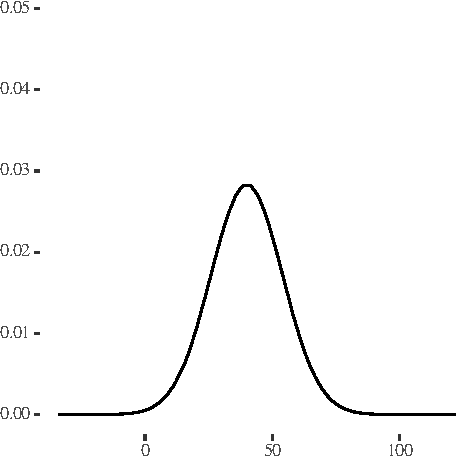
\includegraphics[width=0.8\linewidth]{DegreeOfFreedum_files/figure-latex/unnamed-chunk-5-1} 

}

\caption[標本標準偏差の補正値(不偏推定値)と母平均による標準偏差の差]{標本標準偏差の補正値(不偏推定値)と母平均による標準偏差の差}\label{fig:unnamed-chunk-5}
\end{figure}

\newpage

\hypertarget{ux304aux308fux308aux306b}{%
\section{\texorpdfstring{\textbf{おわりに}}{おわりに}}\label{ux304aux308fux308aux306b}}

 詳細で理論的な説明が必要な場合は『なぜ不偏分散は N-1
で割るのか』\citep{estpdf82:online}を参照してください。  \\
ちなみに母集団(\(x\))の平均値(\(mu\))と標準偏差(\(s\))は以下の通りでした。

\begin{Shaded}
\begin{Highlighting}[numbers=left,,]
\FunctionTok{mean}\NormalTok{(x)                }\CommentTok{\# 平均値}
\end{Highlighting}
\end{Shaded}

\begin{verbatim}
## [1] 3.984684
\end{verbatim}

\begin{Shaded}
\begin{Highlighting}[numbers=left,,]
\NormalTok{(n }\SpecialCharTok{/}\NormalTok{ (n }\SpecialCharTok{{-}} \DecValTok{1}\NormalTok{)) }\SpecialCharTok{*} \FunctionTok{sd}\NormalTok{(x)  }\CommentTok{\# 標準偏差}
\end{Highlighting}
\end{Shaded}

\begin{verbatim}
## [1] 3.0058
\end{verbatim}

 

\bibliography{bib/references.bib}



\end{document}
